%
% wavelets.tex -- Wavelets auf Graphen
%
% (c) 2020 Prof Dr Andreas Müller, Hochschule Rapperswil
%
\section{Wavelets auf Graphen
\label{buch:section:wavelets-auf-graphen}}
\rhead{Wavelets auf Graphen}
In Abschnitt~\ref{buch:subsection:standardbasis-und-eigenbasis} wurde
gezeigt dass die Standardbasis den Zusammenhang zwischen den einzelnen
Teilen des Graphen völlig ignoriert, während die Eigenbasis Wellen
beschreibt, die mit vergleichbarer Amplitude sich über den ganzen
Graphen entsprechen.
Die Eigenbasis unterdrückt also die ``Individualität'' der einzelnen
Knoten fast vollständig.

Wenn man einen Standardbasisvektor in einem Knoten $i$
als Anfangstemperaturverteilung verwendet, erwartet man eine Lösung,
die für kleine Zeiten $t$ die Energie immer in der Nähe des Knotens $i$
konzentriert hat.
Weder die Standardbasis noch die Eigenbasis haben diese Eigenschaft.

\subsection{Vergleich mit der Wärmeleitung auf $\mathbb{R}$}
Ein ähnliches Phänomen findet man bei der Wärmeausbreitung gemäss
der partiellen Differentialgleichung
\[
\frac{\partial T}{\partial t} = -\kappa \frac{\partial^2 T}{\partial x^2}.
\]
Die von Fourier erfundene Methode, die Fourier-Theorie, verwendet die
Funktionen $e^{ik x}$, die Eigenvektoren der zweiten Ableitung
$\partial^2/\partial x^2$ sind.
Diese haben das gleiche Problem, der Betrag von $e^{ikx}$ ist $1$, die
Entfernung von einem Punkt spielt überhaupt keine Rolle.
Die Funktion
\[
F(x,t)
=
\frac{1}{\sqrt{4\pi\kappa t}}e^{-x^2/4\kappa t}
\]
ist eine Lösung der Wärmeleitungsgleichung mit einem Maximum an
der Stelle $0$.
Sie heisst die Fundamentallösung der Wärmeleitungsgleichung.
Durch Überlagerung von Translaten in eine Funktion
\begin{equation}
f(x,t)
=
\int_{-\infty}^\infty f(\xi) F(x-\xi,t)\,d\xi
\label{buch:graphen:eqn:fundamentalueberlagerung}
\end{equation}
kann man die allgemeine Lösung aus Fundamentallösungen zusammensetzen.
Die Fundamentallösungen $f(x-\xi,t)$ sind für kleine Zeiten immer noch
deutlich in einer Umgebung von $\xi$ konzentriert.

% XXX Ausbreitung der Fundamentallösung illustrieren
\begin{figure}
\centering
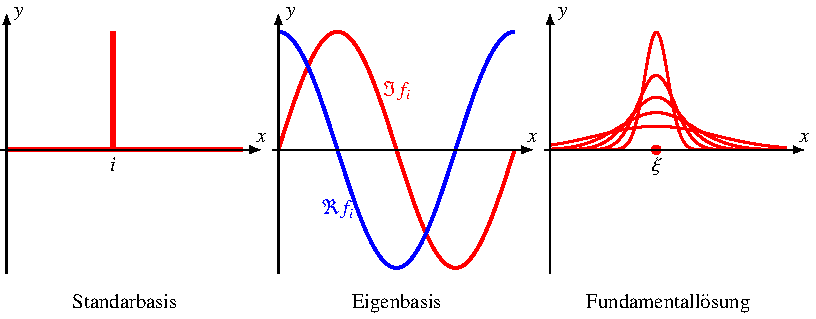
\includegraphics{chapters/70-graphen/images/fundamental.pdf}
\caption{Vergleich der verschiedenen Funktionenfamilien, mit denen
Lösungenfunktionen durch Linearkombination erzeugt werden können.
In der Standarbasis (links) ist es am einfachsten, die Funktionswerte
abzulesen, in der Eigenbasis (Mitte) kann die zeitliche Entwicklung
besonders leicht berechnet werden.
Dazuwischen liegen die Fundamentallösungen (rechts), die eine einigermassen
übersichtliche Zeitentwicklung haben, die Berechnung der Temperatur an 
einer Stelle $x$ zur Zeit $t$ ist aber erst durch das Integral
\eqref{buch:graphen:eqn:fundamentalueberlagerung} gegeben.
\label{buch:graphen:fig:fundamental}}
\end{figure}

\subsection{Fundamentallösungen auf einem Graphen}
Die Wärmeleitungsgleichung auf einem Graphen kann für einen
Standardbasisvektor mit Hilfe der
Lösungsformel~\eqref{buch:graphen:eqn:eigloesung}
gefunden werden.
Aus physikalischen Gründen ist aber offensichtlich, dass die
Wärmeenergie Fundamentallösungen $F_i(t)$ für kurze Zeiten $t$
in der Nähe des Knoten $i$ konzentriert ist.
Dies ist aber aus der expliziten Formel
\begin{equation}
F_i(t)
=
\sum_{j=1}^n \langle f_j,e_i\rangle e^{-\kappa \lambda_i t} f_j
=
\sum_{j=1}^n \overline{f}_{ji} e^{-\kappa \lambda_i t},
\label{buch:graphen:eqn:fundamentalgraph}
\end{equation}
nicht unmittelbar erkennbar.

Man kann aber aus~\eqref{buch:graphen:eqn:fundamentalgraph} ablesen,
dass für zunehmende Zeit die hohen Frequenzen sehr schnell gedämpft
werden.
Die hohen Frequenzen erzeugen also den scharfen Peak für Zeiten nahe
beim Knoten $i$, die zu kleineren $\lambda_i$ beschreiben die Ausbreitung
über grössere Distanzen.
Die Fundamentallösung interpoliert also in einem gewissen Sinne zwischen
den Extremen der Standardbasis und der Eigenbasis.
Die ``Interpolation'' geht von der Differentialgleichung aus,
sie ist nicht einfach nur ein Filter, der die verschiedenen Frequenzen
auf die gleiche Art bearbeitet.

Gesucht ist eine Methode, eine Familie von Vektoren zu finden,
aus der sich alle Vektoren linear kombinieren lassen, in der aber
auch auf die für die Anwendung interessante Längenskala angepasste
Funktionen gefunden werden können.

\subsection{Wavelets und Frequenzspektrum}
Eine Wavelet-Basis der Funktionen auf $\mathbb{R}$ zerlegt


\subsection{Frequenzspektrum
\label{buch:subsection:frequenzspektrum}}
Die Fundamentallösung der Wärmeleitunsgleichung haben ein Spektrum, welches
wie $e^{-k^2}$ gegen $0$ geht.

Die Fundamentallösung entsteht dadurch, dass die hohen Frequenzen
schneller dämpft als die tiefen Frequenzen.


\subsection{Wavelet-Basen
\label{buch:subsection:}}





